
	
	


Another way to evaluate the different nets is to play against them. To do this, we wrote a script called $human\_v\_model.py$ which lets you choose which model to play against. Below we will show you what each model's game against me looked like. For all of the images below, I tried to follow roughly the same moveset so that we could see how the bots reacted differently. I went first each time, so I was the X's and the bot was the O's:

First up, we will play a completely random bot. This bot will pick one of the available spaces to play using a random integer generator. 
\begin{figure}[H]
	\centering
	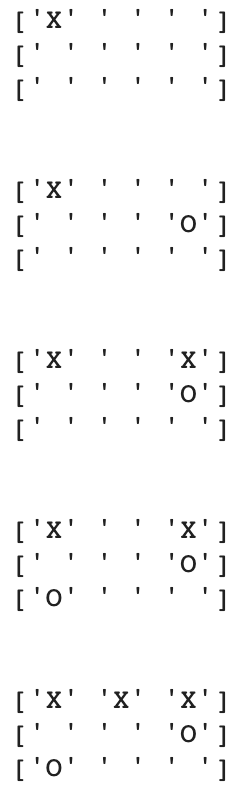
\includegraphics[scale=.3]{h_v_random}
\end{figure}
As you can see, this does not perform well. Because it's random, it doesn't identify any potential defensive moves or offensive moves.

Next up, we will play our Dense Neural Network. We expect that this bot will at the very least play some defensive moves to extend the game a little longer. 

\begin{figure}[H]
	\centering
	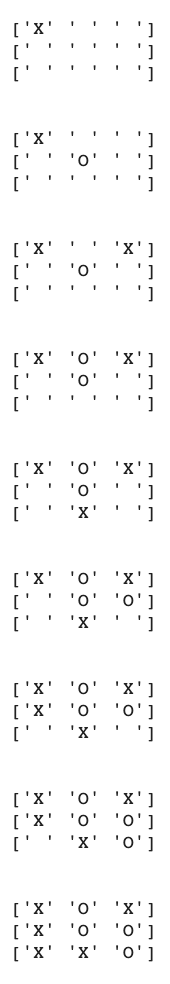
\includegraphics[scale=.3]{h_v_dense}
\end{figure}

First of all, we can see that the bot recognizes that it needs to play at row 2, column 1 to block my first attempt to win. It then recognizes that it should play somewhere in column 2 on its next move so that it has a chance to win if I fail to block it. If it were to play somewhere in column 3 here, it would have no chance to win. After I blocked this, though, is where the bot seems to mess up. For some reason it doesn't identify that I have two in a row and fails to block me, resulting in me winning.

Now we will play our Convolutional Neural Network. This bot performed better statistically when playing the two other bots, so hopefully we see some better performance here. 

\begin{figure}[H]
	\centering
	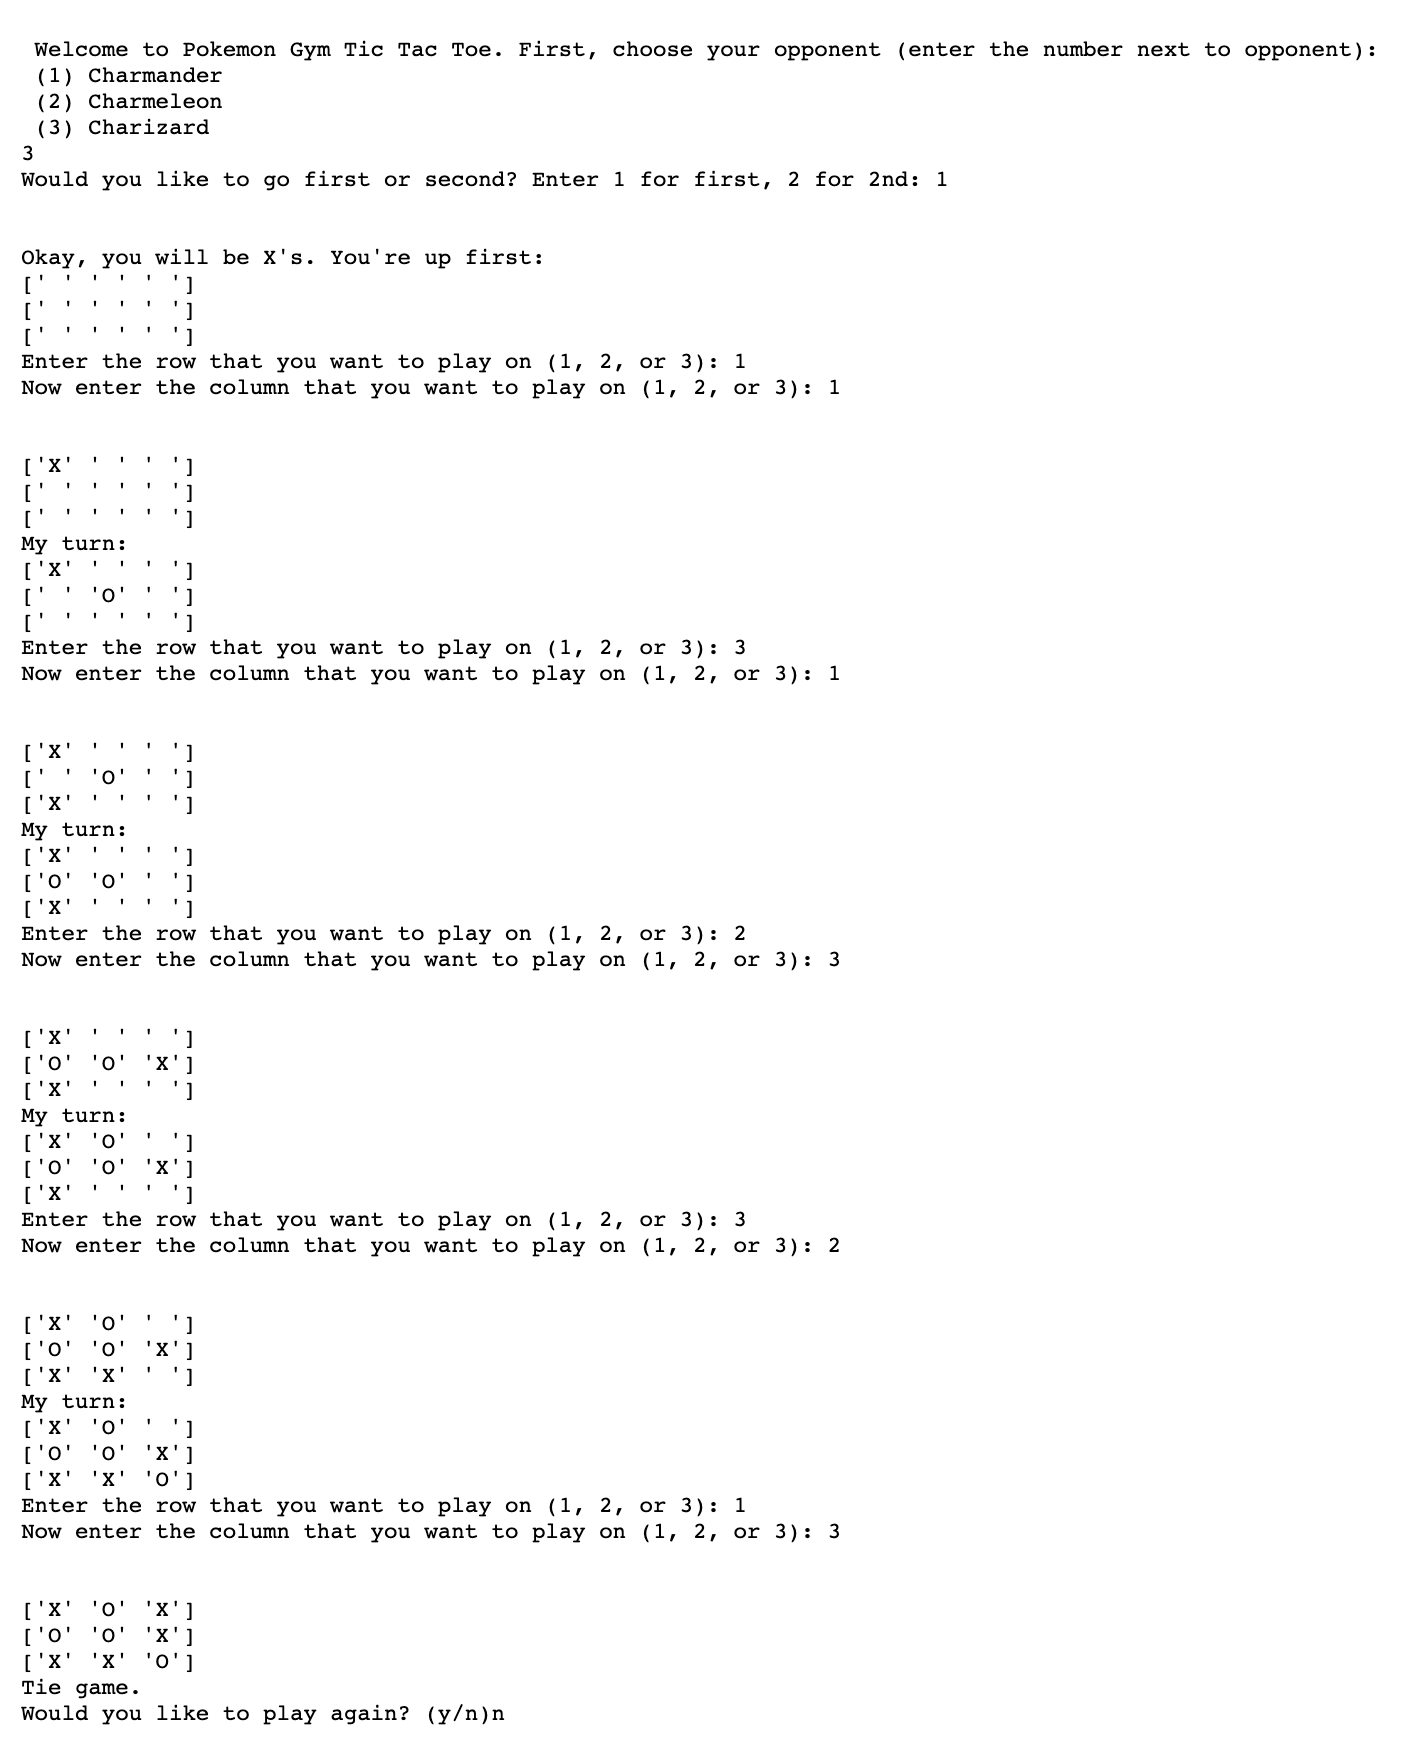
\includegraphics[scale=.3]{h_v_conv}
\end{figure}

Like the DNN bot, this bot identifies follows its best strategy early in the game. We can see, however, that this bot correctly identifies my final chance to win and blocks it, resulting in a tie game. 

